\documentclass{article}
\usepackage{amsmath}
\usepackage{float}
\usepackage{graphicx}

\title{Logistic Regression}
\author{Ta Quang Minh}
\date{\today}

\begin{document}

\maketitle

\section{Introduction}
Inspite of its name, Logistic regression is a statistical method used for binary classification tasks, rather than a regression method. Unlike linear regression, which predicts continuous values, logistic regression predicts the probability that an instance belongs to a particular class. It is widely used in various fields such as healthcare, finance, marketing, and social sciences.

\section{Mathematical forumalation}
Logistic regression models the probability that a binary outcome variable \( Y \) belongs to a particular class based on one or more independent variables \( X \). It uses the logistic function (sigmoid function) to map the linear combination of the independent variables to the probability of the outcome:
\[
P(Y=1|X) = \frac{1}{1 + e^{-(\beta_0 + \beta_1 X_1 + \ldots + \beta_n X_n)}}
\]
Where:
\begin{itemize}
    \item \( P(Y=1|X) \) is the probability that \( Y \) equals 1 given the values of \( X \).
    \item \( \beta_0, \beta_1, \ldots, \beta_n \) are the coefficients (parameters) of the model.
    \item \( X_1, X_2, \ldots, X_n \) are the independent variables.
    \item \( e \) is the base of the natural logarithm.
\end{itemize}

In logistic regression, the model is trained by optimizing a loss function known as the binary cross-entropy (also called log loss) or logistic loss function. This loss function quantifies the difference between the predicted probabilities and the true binary labels.

Let's denote:
\begin{itemize}
    \item \( y_i \) as the true binary label (0 or 1) for the \( i \)-th observation.
    \item \( p_i \) as the predicted probability that the \( i \)-th observation belongs to class 1.
\end{itemize}

The binary cross-entropy loss for logistic regression is defined as:
\[
\text{Binary Cross-Entropy Loss} = -\frac{1}{N} \sum_{i=1}^{N} \left[ y_i \log(p_i) + (1 - y_i) \log(1 - p_i) \right]
\]

Where:
\begin{itemize}
    \item \( N \) is the total number of observations.
    \item \( \log \) denotes the natural logarithm.
\end{itemize}

The goal during training is to minimize this loss function, typically using optimization algorithms such as gradient descent or its variants. The binary cross-entropy loss is a convex function, ensuring that gradient-based optimization methods converge to a global minimum.

The loss can also be interpreted as the inverse of the log-likelihood of the predicted distribution given by the logistic function (in which case we want to maximize the likelihood).

\section{Decision Boundary of Logistic Regression}

In logistic regression with two classes (binary classification), the decision boundary is determined by the coefficients (parameters) of the model. It is either a line in two-dimensional space (for two features) or a hyperplane in higher-dimensional space (for more than two features). Hence logistic regression belongs to the class of linear classifier, and it can not work well with non-linear separable data.

In the case that there are two features \( X_1 \) and \( X_2 \), the decision boundary is given by the equation:
\[
\beta_0 + \beta_1 X_1 + \beta_2 X_2 = 0
\]

\section{Example}

The dataset used in this experiment was generated using the make\_blobs function from scikit-learn. It contains 200 samples with two features and two classes.

The logistic regression model was trained on 80\% of the data and tested on the remaining 20\%. 

\begin{figure}[H]
    \centering
    \resizebox{\textwidth}{!}{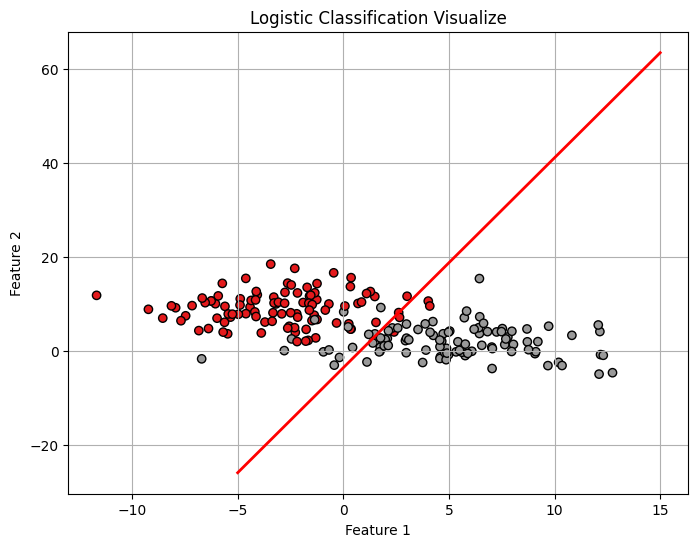
\includegraphics{logis.png}}
    \caption{Logistic Regression}
    \label{fig:example}
\end{figure}

We compared the predicted value of the test set with the true value to get the following classification report.

\begin{table}[h]
\centering
\begin{tabular}{lcccc}
\hline
\textbf{Class} & \textbf{Precision} & \textbf{Recall} & \textbf{F1-Score} & \textbf{Support} \\ \hline
0              & 0.96               & 1.00            & 0.98               & 23               \\
1              & 1.00               & 0.94            & 0.97               & 17               \\ \hline
\textbf{Accuracy}   &                    &                 &                    & 0.97             \\
\textbf{Macro Avg}  & 0.98               & 0.97            & 0.97               & 40               \\
\textbf{Weighted Avg} & 0.98             & 0.97            & 0.97               & 40               \\ \hline
\end{tabular}
\caption{Classification Report}
\label{tab:classification_report}
\end{table}

\section{Applications of Logistic Regression}
Logistic regression finds applications in various domains, including:
\begin{itemize}
    \item \textbf{Medical Diagnosis:} Predicting the likelihood of a patient having a particular disease based on symptoms and test results.
    \item \textbf{Credit Scoring:} Assessing the creditworthiness of individuals based on their financial attributes.
    \item \textbf{Customer Churn Prediction:} Predicting whether a customer will churn (leave) a service based on their behavior and demographics.
    \item \textbf{Sentiment Analysis:} Classifying text data (e.g., reviews, tweets) as positive or negative sentiment.
\end{itemize}

\section{Advantages of Logistic Regression}
Logistic regression offers several advantages, including:
\begin{itemize}
    \item \textbf{Interpretability:} The coefficients in logistic regression provide insights into the relationship between the independent variables and the probability of the outcome.
    \item \textbf{Efficiency:} Logistic regression is computationally efficient and can handle large datasets with relatively low computational resources.
    \item \textbf{Probability Output:} Logistic regression provides probabilistic predictions, allowing for flexible decision-making thresholds.
\end{itemize}

\section{Limitations of Logistic Regression}
Despite its advantages, logistic regression has some limitations:
\begin{itemize}
    \item \textbf{Assumption of Linearity:} Logistic regression assumes a linear relationship between the independent variables and the log odds of the outcome, which may not always hold true.
    \item \textbf{Binary Outcome:} Logistic regression is limited to binary classification tasks and cannot be directly applied to multi-class classification problems without modifications.
    \item \textbf{Sensitivity to Outliers:} Logistic regression can be sensitive to outliers, which may affect model performance.
\end{itemize}

\section{Extensions of Logistic Regression}
Several extensions of logistic regression exist to address its limitations and cater to more complex scenarios, including:
\begin{itemize}
    \item \textbf{Multinomial Logistic Regression:} Generalizes logistic regression to handle multi-class classification problems. It uses the softmax function instead of the logistic sigmoid function used in binary logistic regression
    \item \textbf{Regularized Logistic Regression:} Introduces regularization terms (e.g., L1, L2 regularization) to prevent overfitting and improve generalization.
    \item \textbf{Ordinal Logistic Regression:} Extends logistic regression to handle ordinal outcome variables with ordered categories.
\end{itemize}

\section{Conclusion}
Logistic regression is a versatile and widely used statistical method for binary classification tasks. By modeling the probability of binary outcomes, logistic regression provides interpretable predictions and can be applied to various real-world problems across different domains. In this report, we have presented an overview of the model, as well as its variants, applications, advantages, and limitations.

\end{document}
